\documentclass[tikz,border=10pt]{standalone}
\usepackage{amsmath}
\usepackage{amssymb}
\usepackage{tikz}
\usetikzlibrary{positioning,shapes.geometric,calc,backgrounds,fit}

\begin{document}

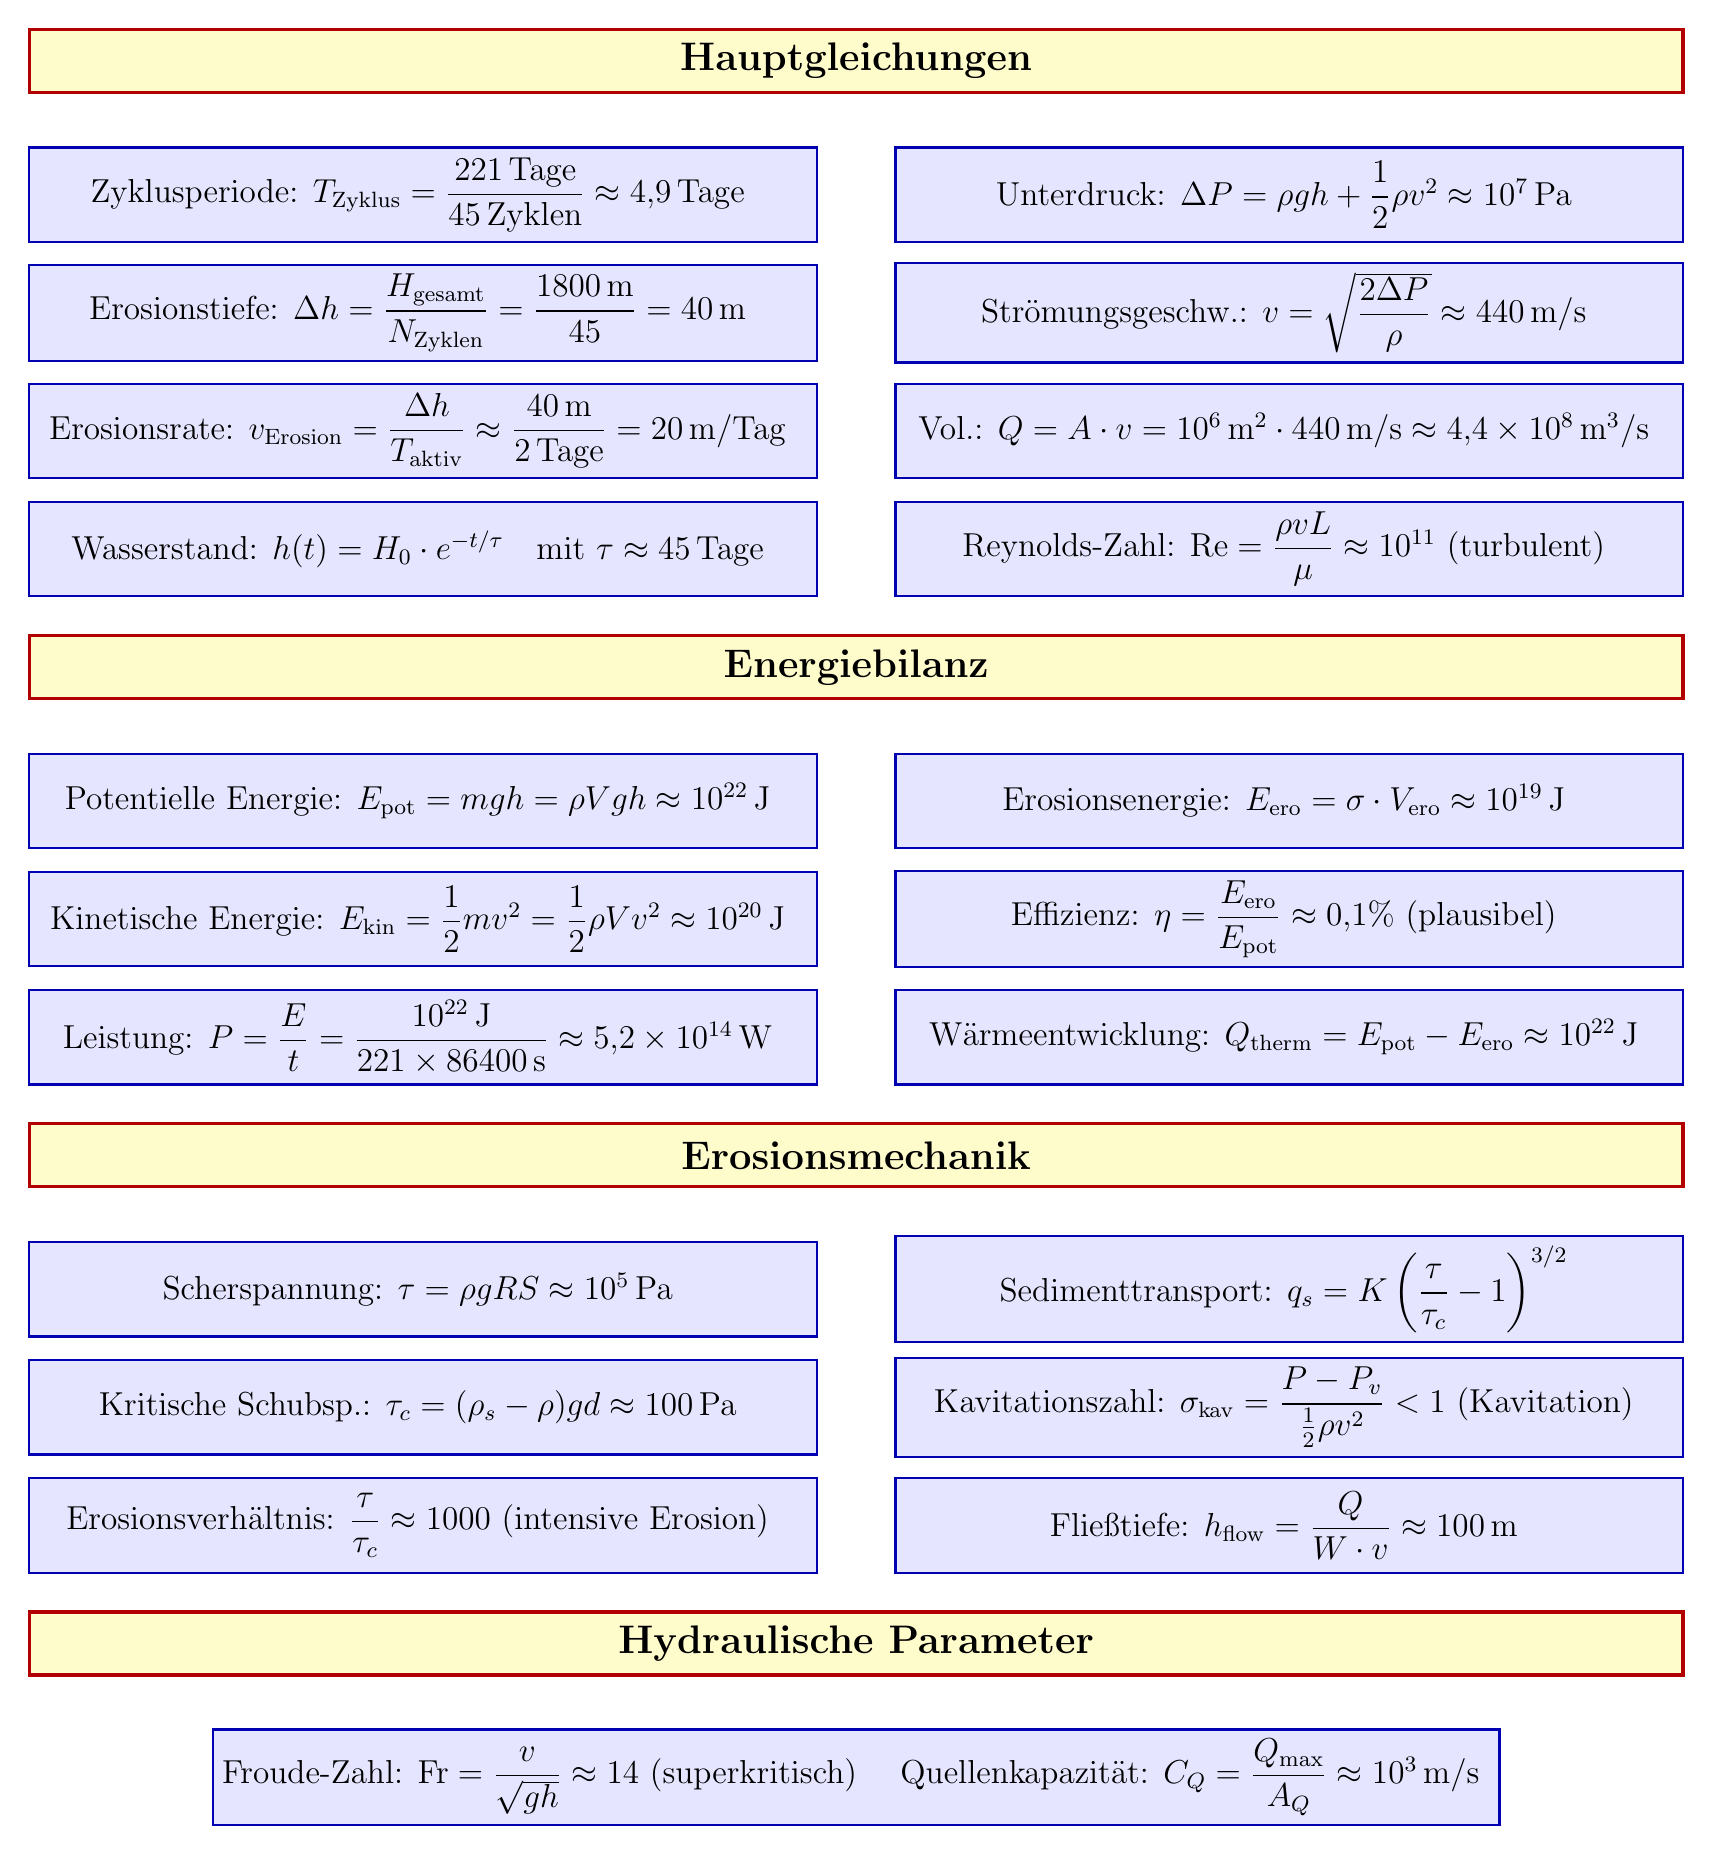
\begin{tikzpicture}[
    formula/.style={
        rectangle,
        draw=blue!70!black,
        fill=blue!10,
        thick,
        minimum width=10cm,
        minimum height=1.2cm,
        align=center,
        font=\large
    },
    section/.style={
        rectangle,
        draw=red!70!black,
        fill=yellow!20,
        very thick,
        minimum width=21cm,
        minimum height=0.8cm,
        align=center,
        font=\Large\bfseries
    },
    title/.style={
        font=\LARGE\bfseries
    }
]

% Title
% \node[title] at (0, 0) {Theoretischer Rahmen: Mathematische Modellierung des Erosionsprozesses};

% Section 1: Hauptgleichungen
\node[section] (sec1) at (0, -1.5) {Hauptgleichungen};

% Left column formulas (Section 1)
\node[formula] (f1) at (-5.5, -3.2) {
    Zyklusperiode: $T_{\mathrm{Zyklus}} = \dfrac{221 \, \mathrm{Tage}}{45 \, \mathrm{Zyklen}} \approx 4{,}9 \, \mathrm{Tage}$
};

\node[formula] (f2) at (-5.5, -4.7) {
    Erosionstiefe: $\Delta h = \dfrac{H_{\mathrm{gesamt}}}{N_{\mathrm{Zyklen}}} = \dfrac{1800 \, \mathrm{m}}{45} = 40 \, \mathrm{m}$
};

\node[formula] (f3) at (-5.5, -6.2) {
    Erosionsrate: $v_{\mathrm{Erosion}} = \dfrac{\Delta h}{T_{\mathrm{aktiv}}} \approx \dfrac{40 \, \mathrm{m}}{2 \, \mathrm{Tage}} = 20 \, \mathrm{m/Tag}$
};

\node[formula] (f4) at (-5.5, -7.7) {
    Wasserstand: $h(t) = H_0 \cdot e^{-t/\tau} \quad \text{mit } \tau \approx 45 \, \mathrm{Tage}$
};

% Right column formulas (Section 1)
\node[formula] (f5) at (5.5, -3.2) {
    Unterdruck: $\Delta P = \rho g h + \dfrac{1}{2}\rho v^2 \approx 10^7 \, \mathrm{Pa}$
};

\node[formula] (f6) at (5.5, -4.7) {
    Strömungsgeschw.: $v = \sqrt{\dfrac{2\Delta P}{\rho}} \approx 440 \, \mathrm{m/s}$
};

\node[formula] (f7) at (5.5, -6.2) {
    Vol.: $Q = A \cdot v = 10^6 \, \mathrm{m}^2 \cdot 440 \, \mathrm{m/s} \approx 4{,}4 \times 10^8 \, \mathrm{m}^3/\mathrm{s}$
};

\node[formula] (f8) at (5.5, -7.7) {
    Reynolds-Zahl: $\mathrm{Re} = \dfrac{\rho v L}{\mu} \approx 10^{11} \text{ (turbulent)}$
};

% Section 2: Energiebilanz
\node[section] (sec2) at (0, -9.2) {Energiebilanz};

% Left column (Section 2)
\node[formula] (f9) at (-5.5, -10.9) {
    Potentielle Energie: $E_{\mathrm{pot}} = m g h = \rho V g h \approx 10^{22} \, \mathrm{J}$
};

\node[formula] (f10) at (-5.5, -12.4) {
    Kinetische Energie: $E_{\mathrm{kin}} = \dfrac{1}{2}m v^2 = \dfrac{1}{2}\rho V v^2 \approx 10^{20} \, \mathrm{J}$
};

\node[formula] (f11) at (-5.5, -13.9) {
    Leistung: $P = \dfrac{E}{t} = \dfrac{10^{22} \, \mathrm{J}}{221 \times 86400 \, \mathrm{s}} \approx 5{,}2 \times 10^{14} \, \mathrm{W}$
};

% Right column (Section 2)
\node[formula] (f12) at (5.5, -10.9) {
    Erosionsenergie: $E_{\mathrm{ero}} = \sigma \cdot V_{\mathrm{ero}} \approx 10^{19} \, \mathrm{J}$
};

\node[formula] (f13) at (5.5, -12.4) {
    Effizienz: $\eta = \dfrac{E_{\mathrm{ero}}}{E_{\mathrm{pot}}} \approx 0{,}1\% \text{ (plausibel)}$
};

\node[formula] (f14) at (5.5, -13.9) {
    Wärmeentwicklung: $Q_{\mathrm{therm}} = E_{\mathrm{pot}} - E_{\mathrm{ero}} \approx 10^{22} \, \mathrm{J}$
};

% Section 3: Erosionsmechanik
\node[section] (sec3) at (0, -15.4) {Erosionsmechanik};

% Left column (Section 3)
\node[formula] (f15) at (-5.5, -17.1) {
    Scherspannung: $\tau = \rho g R S \approx 10^5 \, \mathrm{Pa}$
};

\node[formula] (f16) at (-5.5, -18.6) {
    Kritische Schubsp.: $\tau_c = (\rho_s - \rho) g d \approx 100 \, \mathrm{Pa}$
};

\node[formula] (f17) at (-5.5, -20.1) {
    Erosionsverhältnis: $\dfrac{\tau}{\tau_c} \approx 1000 \text{ (intensive Erosion)}$
};

% Right column (Section 3)
\node[formula] (f18) at (5.5, -17.1) {
    Sedimenttransport: $q_s = K \left(\dfrac{\tau}{\tau_c} - 1\right)^{3/2}$
};

\node[formula] (f19) at (5.5, -18.6) {
    Kavitationszahl: $\sigma_{\mathrm{kav}} = \dfrac{P - P_v}{\frac{1}{2}\rho v^2} < 1 \text{ (Kavitation)}$
};

\node[formula] (f20) at (5.5, -20.1) {
    Fließtiefe: $h_{\mathrm{flow}} = \dfrac{Q}{W \cdot v} \approx 100 \, \mathrm{m}$
};

% Section 4: Hydraulische Parameter (centered at bottom)
\node[section] (sec4) at (0, -21.6) {Hydraulische Parameter};

\node[formula] (f21) at (0, -23.3) {
    Froude-Zahl: $\mathrm{Fr} = \dfrac{v}{\sqrt{g h}} \approx 14 \text{ (superkritisch)}$ \quad
    Quellenkapazität: $C_Q = \dfrac{Q_{\mathrm{max}}}{A_Q} \approx 10^3 \, \mathrm{m/s}$
};

\end{tikzpicture}

\end{document}
